% !TEX root = ./document.tex

\documentclass{article}

\usepackage{mystyle}
\usepackage{myvars}

%-----------------------------

\begin{document}

  \maketitle

  %-----------------------------
  %  TEXT
  %-----------------------------

  \part{Ejercicio Kutner:\\ Mantenimiento de Copiadoras}

    \paragraph{}
    Para la realización del ejercicio de \emph{Mantenimiento de Copiadoras} mediante SAS, lo primero que se ha llevado a cabo es la importación del conjunto de datos a partir del fichero. Para facilitar dicha tarea, se ha realizado una fase previa de preprocesado para convertir el fichero a formato \texttt{csv} denotando por $Y$ la primera columna y $X$ la segunda (tal y como indica el enunciado). Una vez hecho esto, se ha utilizado el fragmento de la figura \ref{code:sas-copiers-1} para importar el conjunto de datos en \emph{SAS}. Por tanto, ya se puede comenzar a realizar el ejercicio.

    \setcounter{section}{1}
    \setcounter{subsection}{19}
    \subsection{\textbf{Copier maintenance}. The Tri-City Office Equipment Corporation sells an imported copier on a franchise basis and performs preventive maintenance and repair service on this copier. The data below have been collected from 45 recent calls on users to perform routine preventive maintenance service; for each call, $X$ is the number of copiers serviced and $Y$ is the total number of minutes spent by the service person. Assume that first-order regression model \eqref{eq:simple-linear-regression-model} is appropriate.}
    \label{sec:e1-20}

      \begin{equation}
      \label{eq:simple-linear-regression-model}
        Y_i = \beta_0 + \beta_1X_i + \varepsilon_i
      \end{equation}

      Analizaremos el modelo de la ecuación \ref{eq:simple-linear-regression-model} mediante un estudio de regresión lineal simple, con $Y_i$ como variable dependiente, $X_i$ como variable independiente, $\beta_0$ como término independiente, y $\beta_1$ como término dependiente o pendiente de la recta de regresión. $\varepsilon_i$ es el error aleatorio que supondremos normal con media $0$ y varianza $\sigma^2$, es decir $\varepsilon_i \sim N(0, \sigma^2)$.


      \subsubsection{Obtain the estimated regression function.}

        \paragraph{}
        Para obtener la generación del modelo de regresión a mediante \emph{SAS} se ha utilizado el fragmento de códido \emph{SAS} de la figura \ref{code:sas-copiers-2}, que calcula los estimadores del modelo de regresión lineal simple que se ilustra en la ecuación \eqref{eq:simple-linear-regression-model}. A partir de dicha sentencia se han obtenido distintas salidas que después han sido utilizadas en otros apartados pedidos por el enunciado del problema.

        \paragraph{}
        Para la resolución de este apartado, ha sido suficiente con consultar el \say{resumen}, que se muestra en la figura \ref{img:copiers-regression-summary}, a partir de la cual se han obtenido los valores de $\beta_0$ y $\beta_1$, que se muestran en las ecuaciones \eqref{eq:beta_0} y \eqref{eq:beta_1} respectivamente.

        \paragraph{}
        Por tanto, la estimación de la función de regresión simple obtenida se muestra en la ecuación \eqref{eq:model_estimation}.

        \begin{figure}[H]
          \centering
          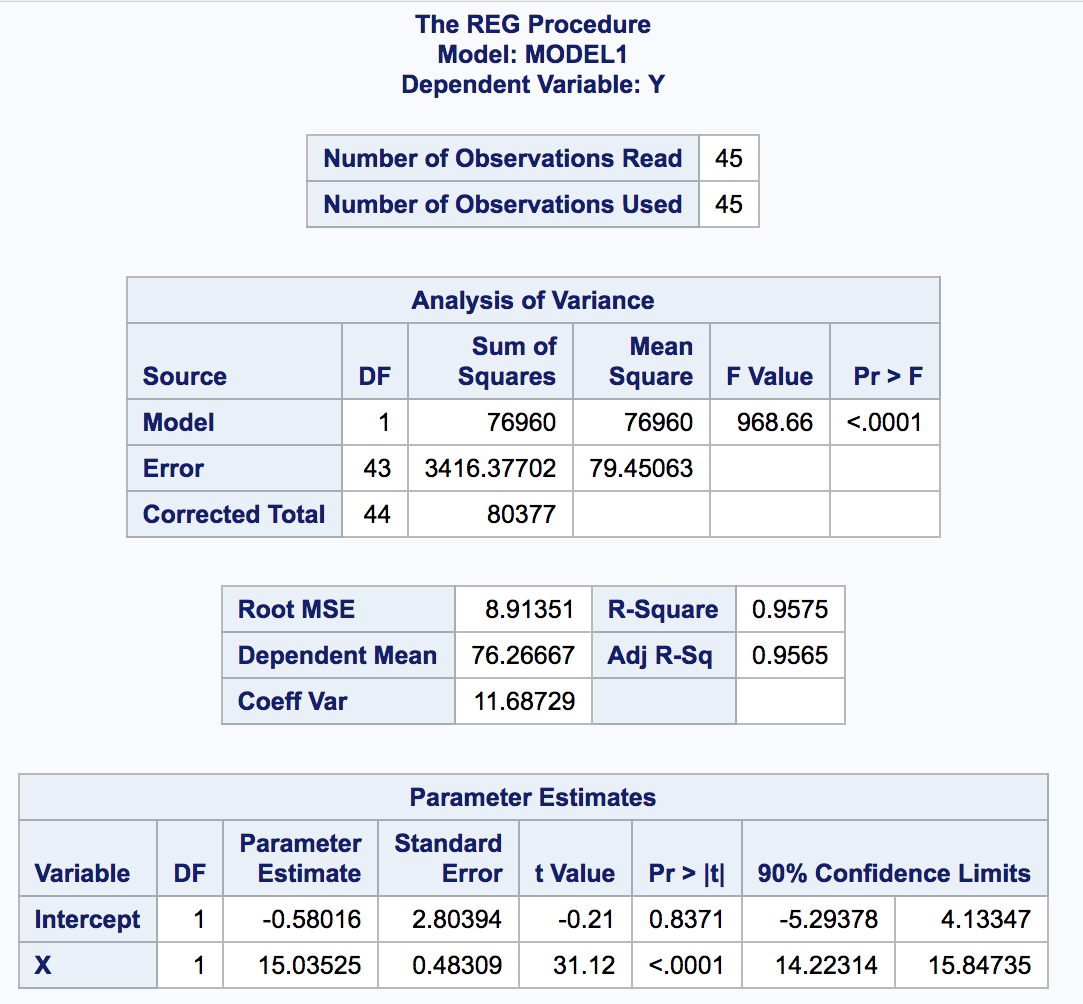
\includegraphics[width=.5\textwidth]{copiers/regression-summary}
          \caption{\emph{Salida SAS}: Mantenimiento de Copiadoras - Resumen de Regresión Lineal Simple}
          \label{img:copiers-regression-summary}
        \end{figure}

        \begin{align}
        \label{eq:beta_0}
          \widehat{\beta}_0 &= -0.58016\\
        \label{eq:beta_1}
          \widehat{\beta}_1 &= 15.03525\\
        \label{eq:model_estimation}
          \widehat{Y_i} &= \widehat{\beta}_0 +\widehat{\beta}_1X_i + \varepsilon_i = -0.58016 + 15.03525 X_i + \varepsilon_i
        \end{align}

      \subsubsection{Plot the estimated regression function and the data. How well does the estimated regression function fit the data?}

        \begin{figure}[H]
          \centering
          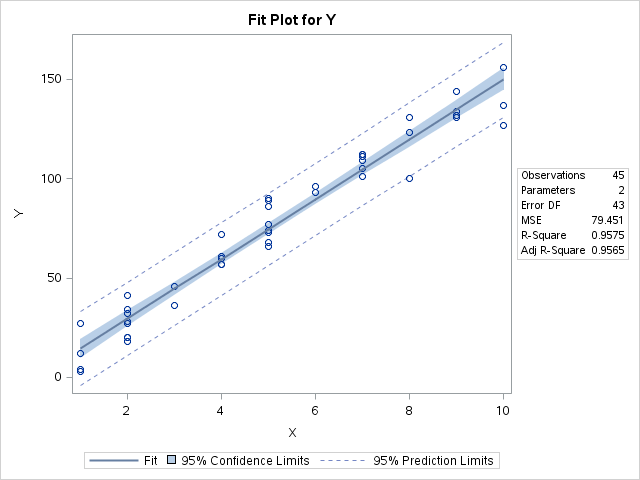
\includegraphics[width=.8\textwidth]{copiers/regression-plot}
          \caption{\emph{Salida SAS}: Mantenimiento de Copiadoras - Gráfico de Regresión Lineal Simple}
          \label{img:copiers-regression-plot}
        \end{figure}

        \paragraph{}
        En este apartado se pide representar la recta de regresión obtenida en el apartado anterior. Afortunadamente, en este caso no ha sido necesaria la utilización de otro fragmento de código, sino que con el utilizado en el apartado anterior (figura \ref{code:sas-copiers-2}) ya se generaba dicho gráfico.

        \paragraph{}
        El gráfico en cuestión se muestra en la figura \ref{img:copiers-regression-plot}, a partir del cual se puede observar la relación lineal existente entre la variable independiente $X$ y la variable dependiente $Y$. Además, se puede apreciar como el modelo de regresión lineal simple se ajusta de manera apropiada a los datos.

        \paragraph{}
        En los siguientes apartados se analizará la dispersión de los datos así como los intervalos de confianza para la media y de predicción. Sim embargo, a simple vista y debido al contexto y unidades de medida de los datos, parece coherente el nivel de dispersión de los datos (variaciones entorno a $10$ minutos entre instalaciones).

      \subsubsection{Interpret $\widehat{\beta}_0$ in your estimated regression function. Does $\widehat{\beta}_0$ provide any relevant information here? Explain.}

        \paragraph{}
        El valor estimado de la ordenada en el origen (o \say{intercept}) se muestra en la ecuación \eqref{eq:beta_0}, el cual está muy próximo al valor $0$. La interpretación del término independiente en este caso podría ser \emph{el número de minutos que se emplean en realizar $0$ mantenimientos}, el cual tiene sentido que esté próximo a $0$ minutos.

        \paragraph{}
        Esto podría deberse a que no se contabiliza el tiempo cuando no hay mantenimiento por hacer, lo cual tiene sentido ya que el estudio trata de analizar la duración del proceso de \emph{mantenimiento de copiadoras}. Algo a destacar es que, posiblemente debido a la muestra patrón utilizada para la generación del modelo, el término independiente ha sido ajustado con valor negativo. Esto no puede tener ninguna interpretación, ya que su valor se ha ajustado de manera que el ajuste global (en términos de mínimos cuadrados) sea mínimo.

        \paragraph{}
        Tal y como se verá en el apartado \ref{sec:copiers-2.5e} del ejercicio \ref{sec:copiers-2.5}, no existen evidencias significativas para asumir que sea distinto de cero. Pero tal y como se discute en dicho apartado, no es apropiado eliminarlo ya que este haría que parte del error explicado por el modelo se convirtiese en error aleatorio, lo cual es algo negativo para el ajuste.


      \subsubsection{Obtain a point estimate of the mean service time when $X = 5$ copiers are serviced.}

        \paragraph{}
        Para la obtención de una estimación puntual para $X=5$, se ha decidido realizar el proceso de añadir una nueva observación al conjunto de datos (de manera que tan solo contenga el valor de la variable independiente $X$). Para ello, se ha utilizado el fragmento de código \emph{SAS} de la figura \ref{code:sas-copiers-3}. Nótese que esto podría haberse llevado a cabo mediante la simple sustitución del valor $X$ en la función de regresión de la ecuación \eqref{eq:model_estimation}, pero esto no nos habría ofrecido una estimación del la varianza.

        \paragraph{}
        Por tanto, la salida obtenida a través de \emph{SAS} se muestra en la figura \ref{img:copiers-regression-prediction}, la cual indica el valor predicho, así como una estimador de la desviación típica respecto de la media en ese punto. Estos valore se muestran en las ecuaciones \eqref{eq:x_5_e} y \eqref{eq:x_5_var}.

        \paragraph{}
        La interpretación que se le puede dar a dichos resultados es que para el mantenimiento de $5$ copiadoras se dedica en torno a $74.6$ minutos con una variación media de $1.15$ minutos.

        \begin{figure}[H]
          \centering
          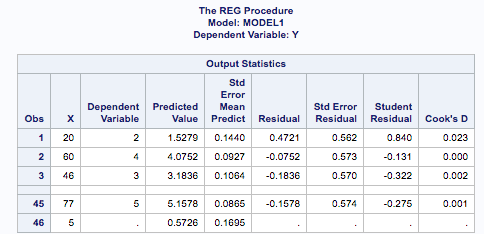
\includegraphics[width=.6\textwidth]{copiers/regression-prediction}
          \caption{\emph{Salida SAS}: Mantenimiento de Copiadoras - Prediccion de Regresión Lineal Simple para $X = 5$}
          \label{img:copiers-regression-prediction}
        \end{figure}

        \begin{align}
        \label{eq:x_5_e}
          \begin{split}
            E\left[\widehat{Y} \mid X = 5\right] &=
            E\left[\widehat{\beta}_0 +\widehat{\beta}_1X + \varepsilon \mid X = 5\right]
            = -0.58016 + 15.03525 * 5 + 0 = 74.5961
          \end{split}\\
        \label{eq:x_5_var}
          \begin{split}
            Var\left[\widehat{Y} \mid X = 5\right] &=
            \sigma^2\left(\frac{1}{n} + \frac{(x^* - \bar{x})^2}{S_{xx}}\right) =
            1.1531 ^ 2 =
            1.3298
          \end{split}
        \end{align}

    \setcounter{subsection}{23}
    \subsection{Refer to \textbf{Copier maintenance} Problem \ref{sec:e1-20}.}

      \subsubsection{Obtain the residuals $e_i$ and the sum of the squared residuals $\sum_i e_i^2$. What is the relation between the sum of the squared residuals here and the quantity $Q$ in \eqref{eq:least-squares-criterion}?}

        \begin{figure}[H]
          \centering
          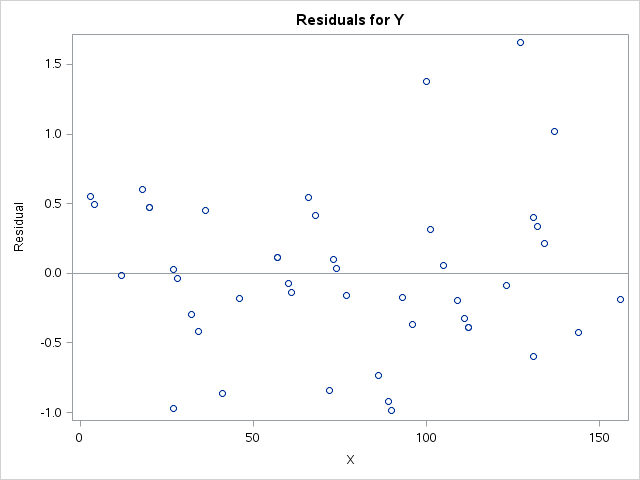
\includegraphics[width=.8\textwidth]{copiers/regression-residuals}
          \caption{\emph{Salida SAS}: Mantenimiento de Copiadoras - Gráfico de Residuos de Regresión Lineal Simple}
          \label{img:copiers-regression-residuals}
        \end{figure}

        \paragraph{}
        En este apartado se pide obtener los residuos $e_i$. Para ello, se ha creido conveniente la representación de un gráfico de resiudos, el cual ha sido obtenido mediante el fragmento de código de la figura \ref{code:sas-copiers-2} utilizado en apartados anteriores.

        \paragraph{}
        Este gráfico de residuos se muestra en la figura \ref{img:copiers-regression-residuals} y a partir de él se puede apreciar una distribución más o menos uniforme de los errores (tiene cierta forma de parábola, pero esta característica es sutil). También se puede apreciar la dispersión de los datos en torno al valor $10$, tal y como se indicó en partaados anteriores.

        \begin{equation}
        \label{eq:least-squares-criterion}
          Q = \sum\limits_{i=1}^n(Y_i - \beta_0 - \beta_1X_i)^2 = 3416.37702
        \end{equation}

        \paragraph{}
        En el título del apartado, también se pide el valor de la suma de errores al cuadrado $\sum_i e_i^2$, así como su relación con el valor $Q$, que se muestra en la ecuación \eqref{eq:least-squares-criterion}. El valor $Q$ es aquel que se trata de minimizar bajo el criterio de mínimos cuadrados en el modelo de regresión simple. Este ha sido extraido del resumen generado por \emph{SAS}, que se muestra en la figura \ref{img:copiers-regression-summary} utilizada en otros apartados.

        \paragraph{}
        Por tanto, es la medida del error en términos de mínimos cuadrados de la recta de regresión obtenida con respecto del conjunto de datos. sto puede escribirse como $Q = \sum_{i=1}^n(Y_i - \widehat{Y}_i)^2$, y dado que los errores $e_i$ se definen como $Y_i - \widehat{Y}_i$ la equivalencia es directa, es decir, $Q = \sum_i e_i^2$.

      \subsubsection{Obtain point estimates of $\sigma^2$ and $\sigma$. In what units is $\sigma$ expressed?}

        \paragraph{}
        En este apartado se han pedido obtener estimaciones acerca de la dispersión de los errores, es decir, del valor $\sigma$. Al igual que en anteriores apartados, este valor se ha obtenido a partir del código \emph{SAS} de la figura \ref{code:sas-copiers-2}, que ha generado los resultados obtenidos en la figura \ref{img:copiers-regression-summary}.

        \paragraph{}
        La varianza y la desviación típica de los errores se muestran en las ecuaciones \eqref{eq:sigma-2} y \eqref{eq:sigma} respectivamente. En el título del apartado se indica además que se explique cuáles son las unidades de medida de la desviación típica de los errores $\sigma$. Es sencillo entender que las unidades de esta medida serán en \emph{minutos}, ya que esta mide la dispersión de los datos en torno a la predicción obtenida por la recta de regresión, la cual se refiere a la variable dependiente $Y$, que representa el número de minutos en realizar el mantenimiento.

        \begin{align}
        \label{eq:sigma-2}
          \begin{split}
            \widehat{\sigma}^2 &= MSE = \frac{SSE}{n-2} = \frac{\sum_{i=1}^n(Y_i - \widehat{Y}_i)^2}{n-2} = \frac{3416.37702}{45-2} = 79.45063
          \end{split} \\
        \label{eq:sigma}
          \begin{split}
            \widehat{\sigma} &= \sqrt{\widehat{\sigma}^2} = \sqrt{79.45063} = 8.91351
          \end{split}
        \end{align}

    \setcounter{section}{2}
    \setcounter{subsection}{4}
    \subsection{Refer to \textbf{Copier maintenance} Problem \ref{sec:e1-20}.}
    \label{sec:copiers-2.5}

      \subsubsection{Estimate the change in the mean service time when the number of copiers serviced increases by one. Use a $90\%$ confidence interval. Interpret your confidence interval.}
      \label{sec:copiers-2.5a}

        \paragraph{}
        El enunciado de este apartado pide que se obtenga un intervalo de confianza del $90\%$ para la estimación de la pendiente de la regresión $\beta_1$. Para ello se ha utilizado la salida obtenida por el fragmento de código de la figura \ref{code:sas-copiers-2}, que se muestra en la figura \ref{img:copiers-regression-summary}.

        \begin{align}
          t_{n-2;1-\frac{\alpha}{2}} &= t_{43;0.95} = 1.681071\\
          Var\left[\widehat{\beta}_1\right] &= 0.23337
        \end{align}

        \paragraph{}
        En esta se aparece el intervalo de confianza al $90\%$ para el valor $\beta_1$, el cual se muestra en la ecuación \eqref{eq:copiers-beta-1-ic}. Este se construye a partir de la estimación $\widehat{\beta}_1=15.03525$, cuyo valor se relaja a partir de un determinado error de estimación $t_{n-2; 1-\frac{\alpha}{2}} \sqrt{Var\left[ \widehat{\beta}_1 \right]} = 1.681071*\sqrt{0.23337} = 0.8121$.

        \begin{equation}
        \label{eq:copiers-beta-1-ic}
          \text{I.Conf.}
          = \left[\widehat{\beta}_1 \pm t_{n-2;1-\frac{\alpha}{2}}\sqrt{Var\left[\widehat{\beta}_1\right]}\right]
          = \left[15.03525 \pm 0.8121\right]
          = \left[14.2232, 15.8474\right]
        \end{equation}

        \paragraph{}
        La interpretación de dicho intervalo es la siguiente: Con una seguridad del $90\%$ el tiempo medio de mantenimiento de cada copiadora se encuentra entre $14.2232$ y $15.8474$ minutos.

      \subsubsection{Conduct a \emph{t-test} to determine whether or not there is a linear association between $X$ and $Y$ here; control the $\alpha$ risk at $0.1$. State the alternatives, decision rule, and conclusion. What is the \emph{P-value} of your test?}
      \label{sec:copiers-2.5b}

        \paragraph{}
        En este apartado se pide realizar un test de hipótesis acerca de la existencia de asociación entre $X$ e $Y$. Es decir, si la pendiente de nuestra recta de regresión puede ser considerada nula. Para ello, se puede modelar el test de hipótesis tal y como se indica en la ecuación \eqref{eq:copiers-beta1-t-test}.

        \begin{equation}
        \label{eq:copiers-beta1-t-test}
          \begin{split}
            H_0&: \beta_1 = 0 \\
            H_1&: \beta_1 \neq 0
          \end{split}
        \end{equation}

        \paragraph{}
        En este caso se pide realizar el test de hipótesis mediante el procedimiento de \emph{test t} (ya que en la sección \ref{sec:copiers-2.24b} del ejercicio \ref{sec:copiers-2.24} se pide realizar el mismo test, pero esta vez a partir de la distribución $F$, para comprobar su equivalencia). El \emph{p-valor} de este test se obtiene tal y como se indica en la ecuación \eqref{eq:copiers-beta1-p-value}. Por ser un test de \emph{2 vías} se toma el valor absoluto y se multiplica por 2 el valor de probabilidad ($\alpha/2$ a cada lado). Para ello se ha utilizado la salida obtenida por el fragmento de código de la figura \ref{code:sas-copiers-2}, que se muestra en la figura \ref{img:copiers-regression-summary}.

        \begin{equation}
        \label{eq:copiers-beta1-p-value}
          \text{p-value}
          = 2Pr\left[\abs{\frac{\widehat{\beta}_1 - 0}{\sqrt{Var\left[\widehat{\beta}_1\right]}}} > t_{n-2}\right]
          = 2Pr\left[\frac{15.03525}{0.48309} > t_{43}\right]
          = 2Pr\left[31.12 > t_{43}\right]
          < 0.0001
        \end{equation}

        \paragraph{}
        El \emph{p-valor} obtenido es muy próximo a $0$, por lo que a nivel $\alpha = 0.1$ nos vemos obligados a rechazar la hipótesis de que $\beta_1$ es nulo. Esto quiere decir por tanto que asumiremos que existe relación lineal entre el $X$ e $Y$.

      \subsubsection{Are your results in parts (\ref{sec:copiers-2.5a}) and (\ref{sec:copiers-2.5b}) consistent? Explain.}

        \paragraph{}
        En este caso se nos pide analizar los resultados obtenidos en los dos últimos apartados para comprobar si son coherentes entre sí, ya que ambos se refieren a procesos de inferencia sobre la estimación de $\widehat{\beta}_1$.

        \paragraph{}
        Los resultados si que son coherentes entre sí, ya que en el primero de ellos se ha calculado un intervalo de confianza (o aceptación) para el valor de la pendiente $\beta_1$ de la regresión, mientras que en el siguiente caso se ha realizado un test sobre el valor de dicha pendiente (si se puede tomar como nula). Puesto que en el primer caso el límite izquierdo del intervalo se encuentra en torno al valor $14$ con un nivel de confianza del $90\%$, es razonable que sobre el mismo nivel de confianza se tenga que rechazar la hipótesis de que el valor $0$ está incluido en dicho intervalo de aceptación.

      \subsubsection{The manufacturer has suggested that the mean required time should not increase by more
than $14$ minutes for each additional copier that is serviced on a service call. Conduct a test to decide whether this standard is being satisfied by Tri-City. Control the risk of a Type I error at $0.05$. State the alternatives, decision rule, and conclusion. What is the \emph{P-value} of the test?}

        \paragraph{}
        En este caso se pide realizar un test de hipótesis acerca de un intervalo, referido una vez más al valor de la pendiente de la relación $\beta_1$. Un fabricante quiere comprobar si es razonable asumir que el tiempo de mantenimiento de una copiadora es menor que $14$ minutos con un nivel de confianza del $95\%$. Por tanto. el test de hipótesis se define tal y como se indica en la ecuación \eqref{eq:copiers-beta1-t-test-interval}.

        \begin{equation}
        \label{eq:copiers-beta1-t-test-interval}
          \begin{split}
            H_0&: \beta_1 \leq 14 \\
            H_1&: \beta_1 > 14
          \end{split}
        \end{equation}

        \paragraph{}
        En este caso para la realización del \emph{test t}, ya no hay que selecciona $\alpha/2$ a cada lado, ya que que el test es de \emph{1 vía}. El \emph{p-valor} del test se ha obtenido tal y como se indica en la ecuación \eqref{eq:copiers-beta1-p-value-interval}.

        \begin{equation}
          \label{eq:copiers-beta1-p-value-interval}
            \text{p-value}
            = Pr\left[\frac{\widehat{\beta}_1 - 14}{\sqrt{Var\left[\widehat{\beta}_1\right]}} > t_{n-2}\right]
            = Pr\left[\frac{1.03525}{0.48309} > t_{43}\right]
            = Pr\left[2.14297 > t_{43}\right]
            = 0.01890824
        \end{equation}

        \paragraph{}
        El \emph{p-valor} en este caso, no es tan próximo a $0$ como en anteriores tests. Sin embargo, con un nivel de confianza del $95\%$ nos vemos obligados a rechazar la hipótesis de que $\beta_1$ sea menor que $14$. Nótese que esto no se puede rechazar con un nivel de confianza del $99\%$.

      \subsubsection{Does $\widehat{\beta}_0$ give any relevant information here about the start-up time on calls-i.e., about the time required before service work is begun on the copiers at a customer location?}
      \label{sec:copiers-2.5e}

        \paragraph{}
        En este apartado se pide realizar un test de hipótesis que permita comprobar si el valor $\beta_0$ es nulo. Esto puede interpretarse como que el tiempo para realizar $0$ mantenimientos de copiadoras también es $0$. El test se plantea por tanto como se indica en la ecuación \eqref{eq:copiers-beta0-t-test}.

        \begin{equation}
          \label{eq:copiers-beta0-t-test}
          \begin{split}
            H_0&: \beta_0 = 0 \\
            H_1&: \beta_0 \neq 0
          \end{split}
        \end{equation}

        \paragraph{}
        Para la realización de dicho test de hipótesis se ha calculado el \emph{p-valor} tal y como se indica en la ecuación \eqref{eq:copiers-beta0-p-value}, que tal y como ocurría en el análogo de $\beta_1$, se plantea como un test de \emph{2 vías} por lo que se toma el valor absoluto y se multiplica por $2$ (debido a la simetría de la distribución $t$). Para ello se ha utilizado la salida obtenida por el fragmento de código de la figura \ref{code:sas-copiers-2}, que se muestra en la figura \ref{img:copiers-regression-summary}.

        \begin{equation}
          \label{eq:copiers-beta0-p-value}
            \text{p-value}
            = 2Pr\left[\abs{\frac{\widehat{\beta}_0 - 0}{\sqrt{Var\left[\widehat{\beta}_0\right]}}} > t_{n-2}\right]
            = 2Pr\left[\abs{\frac{-0.58016}{2.80394}} > t_{43}\right]
            = 2Pr\left[\abs{-0.21} > t_{43} \right]
            = 0.8371
        \end{equation}

        \paragraph{}
        Debido al elevado valor obtenido en el \emph{p-valor} estamos en condiciones suficientes como para aceptar la hipótesis nula de la ecuación \eqref{eq:copiers-beta0-t-test}, que nos indica que el valor de la ordenada en el origen es $0$. Esto puede interpretarse como que cuando no se realiza ningún mantenimiento, tampoco se dedica ningún minuto.

        \paragraph{}
        Sin embargo, no tiene ningún sentido eliminar el estimador $\widehat{\beta}_0$ del modelo, puesto que su valor (muy próximo a cero pero no cero) permite que la recta haya sido ajustada a los datos de manera óptima, y su eliminación tan solo perjudicaría la minimización cuadrática del error del modelo.

    \setcounter{subsection}{13}
    \subsection{Refer to \textbf{Copier maintenance} Problem \ref{sec:e1-20}.}

      \begin{figure}[H]
        \centering
        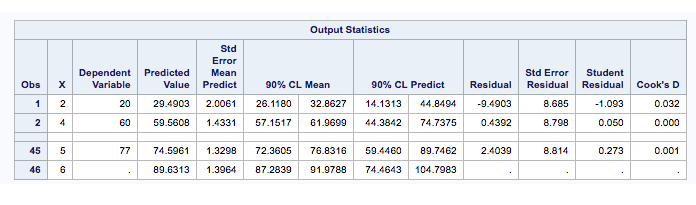
\includegraphics[width=.85\textwidth]{copiers/regression-prediction2}
        \caption{\emph{Salida SAS}: Mantenimiento de Copiadoras - Prediccion de Regresión Lineal Simple para $X = 6$}
        \label{img:copiers-regression-prediction2}
      \end{figure}

      \subsubsection{Obtain a $90\%$ confidence interval for the mean service time on calls in which six copiers are serviced. Interpret your confidence interval.}
      \label{sec:copiers-2.14a}

        \paragraph{}
        En este apartado, se pide obtener un intervalo de confianza del $90\%$ para la media de la variable dependiente $Y$ cuando la variable dependiente toma el valor $X=6$. Para ello, se ha utilizado el fragmento de código \emph{SAS} incluido en la figura \ref{code:sas-copiers-4}, a partil del cual se ha obtenido la salida de la figura \ref{img:copiers-regression-prediction2}.

        \begin{align}
          E[\widehat{Y}_h] &= E[\widehat{\beta}_0 +\widehat{\beta}_1 * 6 + \varepsilon_h] = 89.6313\\
          t_{n-2;1-\frac{\alpha}{2}} &= t_{43;0.95} = 1.681071\\
          Var\left[\widehat{Y}_h \right]  &= 1.9499
        \end{align}

        \paragraph{}
        El resultado del intervalo de confianza para la media se muestra en la ecuación \eqref{eq:copiers-pred-6-ic}.

        \begin{equation}
        \label{eq:copiers-pred-6-ic}
          \text{I.Conf.}
          = \left[E[\widehat{Y}_h] \pm t_{n-2;1-\frac{\alpha}{2}}\sqrt{Var\left[\widehat{Y}_h \right]}\right]
          = \left[89.6313 \pm 2.3475\right]
          = \left[87.2839, 91.9788\right]
        \end{equation}

      \subsubsection{Obtain a $90\%$ prediction interval for the service time on the next call in which six copiers are serviced. Is your prediction interval wider than the corresponding confidence interval in part (\ref{sec:copiers-2.14a})? Should it be?}

        \paragraph{}
        En este apartado, se pide obtener un intervalo de predicción del $90\%$ para la media de la variable dependiente $Y$ cuando la variable dependiente toma el valor $X=6$. Para ello, se ha utilizado el fragmento de código \emph{SAS} incluido en la figura \ref{code:sas-copiers-4}, a partil del cual se ha obtenido la salida de la figura \ref{img:copiers-regression-prediction2}.

        \begin{align}
          E[\widehat{Y}_{pred}] &= E[\widehat{\beta}_0 +\widehat{\beta}_16 + \varepsilon_i] = 89.6313\\
          t_{n-2;1-\frac{\alpha}{2}} &= t_{43;0.95} = 1.681071\\
          Var\left[\widehat{Y}_{pred}\right] &= \widehat{\sigma}^2 + Var\left[\widehat{Y}_h \right]  =79.45063 + 1.9499 = 81.40053
        \end{align}

        \paragraph{}
        El resultado del intervalo de predicción se muestra en la ecuación \eqref{eq:copiers-pred-6-ipred}.

        \begin{equation}
          \label{eq:copiers-pred-6-ipred}
          \begin{split}
            \text{I.Pred.}
            = \left[E[\widehat{Y}_{pred}] \pm z_{1-\frac{\alpha}{2}}\sqrt{Var\left[\widehat{Y}_{pred}\right]}\right]
            = \left[89.6313 \pm 15.167\right]
            = \left[74.4643, 104.7983\right]
          \end{split}
        \end{equation}

        \paragraph{}
        Tal y como se puede apreciar, el intervalo de predicción es mucho más amplio que el intervalo de confianza para la media. Esto tiene sentido ya que el intervalo de predicción tiene en cuenta la dispersión generada en cada observación, es decir, su varianza tiene un $\widehat{\sigma}^2$ \say{mas} que el intervalo de confianza.

    \setcounter{subsection}{23}
    \subsection{Refer to \textbf{Copier maintenance} Problem \ref{sec:e1-20}.}
    \label{sec:copiers-2.24}

      \setcounter{subsubsection}{1}
      \subsubsection{Conduct an \emph{F-test} to determine whether or not there is a linear association between time spent and number of copiers serviced; use $\alpha = 0.1$. State the alternatives, decision rule, and conclusion.}
      \label{sec:copiers-2.24b}

        \paragraph{}
        En este caso, se pide realizar un test de la $F$ para comprobar si existe relación de dependencia entre la variable dependiente $Y$ y la variable dependiente $X$. Por tanto, esto se puede modelar de la misma manera que se hizo en el apartado \ref{sec:copiers-2.5b} del ejercicio \ref{sec:copiers-2.5}.

        \paragraph{}
        El test de hipótesis que se realizará se muestra en la ecuación \eqref{eq:copiers-h-0-f-test}, el cual es equivalente al del apartado previamente citado. Sin embargo, la manera de proceder para la realización del test, en este caso será diferente. Tal y como se indicó anteriormente, mediante el \emph{test-t} se prueba que la variable de interés tome un determinado valor (lo cual lo hace más general que el que se ha realizado en esta sección).

        \paragraph{}
        En este caso, en lugar de realizar el test directamente sobre la estimación de $\beta_1$, se realiza sobre la variación recogida por el modelo. En concreto, se compara la relación entre la variación recogida por el modelo y la aleatoria con la distribución $F$ con $1$ y $n-2$ grados de libertad, para así obtener el \emph{p-valor} del test.

        \paragraph{}
        Se puede demostar que los resultados obtenidos sobre el test de existencia de correlación entre $X$ e $Y$ son equivalente entre el \emph{test t} y el \emph{test F}

        \begin{equation}
          \label{eq:copiers-h-0-f-test}
          \begin{split}
            H_0&: \beta_1 = 0 \\
            H_1&: \beta_1 \neq 0
          \end{split}
        \end{equation}

        \paragraph{}
        En este caso, se ha obtenido un \emph{p-valor} muy próximo a cero, tal y como se indica en la ecuación \eqref{eq:copiers-f-test-p-value}. Dado que el valor $\alpha$ se ha fijado en $0.1$, nos vemos obligados a rechazar la hipótesis de que el valor de $\beta_1$ es igual a cero. Este resultado es equivalente a obtenido para el \emph{test t}

        \begin{equation}
        \label{eq:copiers-f-test-p-value}
          \text{p-value} = Pr\left[\frac{MSM}{MSE} > F_{1;n-2}\right] =
          Pr\left[\frac{76960}{79.45063} > F_{1;43}\right] =
          Pr\left[968.66 > F_{1;43}\right] <
          0.0001
        \end{equation}

      \subsubsection{By how much, relatively, is the total variation in number of minutes spent on a call-reduced when the number of copiers serviced is introduced into the analysis? Is this a relatively small or large reduction? What is the name of this measure?}

        \paragraph{}
        En este apartado se pide estudiar el grado de variación recogida por el modelo. Dicho grado de variación se puede estudiar a partir del coeficiente de determinación $R^2$, que representa el ratio de variación en términos de suma de cuadrados entre el modelo y el total del conjunto de datos. Por tanto, este siempre toma valores en el intervalo $[0,1]$.

        \paragraph{}
        En este caso, el modelo recoge el $95.74\%$ de la variación del conjunto de datos. Por tanto, se cree que dicho ajuste ha sido acertado. La expresión del coeficiente de determinación se muestra en la ecuación \eqref{eq:copiers-r-2}. Esta ha sido extraida de la figura \ref{img:copiers-regression-summary}, generada a partir del fragmento de código de la figura \ref{code:sas-copiers-2} utilizado en otros apartados.

        \begin{equation}
        \label{eq:copiers-r-2}
          R^2 = \frac{SSM}{SST} = \frac{76960}{76960 + 3416.37702} = 0.9574
        \end{equation}

      \subsubsection{Calculate $r$ and attach the appropriate sign.}

        \paragraph{}
        En este apartado, se pide obtener el coeficiente de correlación entre las variables. Esta medida sirve para cuantizar el grado de relación entre variables, así como si esta relación es positiva o negativa. El coeficiente de correlación toma valores en el interva $[-1,1]$ indicando valores proximos al $1$ una relación lineal fuerte positiva y $-1$ una relación lineal fuerte negativa, mientras que los valores próximos al $0$ indican una relación débil entre las variables.

        \paragraph{}
        Este coeficiente se puede definir como $r=\frac{Cov[X,Y]}{\sqrt{Var[X]Var[Y]}}$, aunque en este caso se ha obtenido mediante la propiedad de la ecuación \eqref{eq:copier-maintante-corr-coef}. Cuando se utiliza esta ecuación es necesario ajustar el signo de manera \say{manual}, ya que el coeficiente de determinación $R^2$ tan solo toma valores positivos.

        \begin{equation}
          \label{eq:copier-maintante-corr-coef}
          r = \pm \sqrt{R^2} = + 0.9785
        \end{equation}

        \paragraph{}
        En este caso, tras analizar los resultados de la ecuación \eqref{eq:copier-maintante-corr-coef} y aplicar el signo positivo (basta con consultar el gráfico de la regresión de la figura \ref{img:copiers-regression-plot} para entender que la relación es positiva), podemos asegurar que existe una fuerte relación entra estas variables.

        \paragraph{}
        Este valor es coherente con la interpretación del conjunto de datos, que relaciona el tiempo de realización de un servicio (en este caso en minutos) con el número de unidades de trabajo que hay que desempeñar en dicho servicio (en este caso el número de copiadoras a las que realizar tareas de mantenimiento).

  \part{Ejercicios Montgomery:}

  \setcounter{section}{2}
  \subsection{En la tabla B.1 del apéndice aparecen datos sobre el desempeño de los 26 equipos de la Liga Nacional de Fútbol en 1976. Se cree que la cantidad de yardas ganadas por tierra por los contrarios ($x_8$) tiene un efecto sobre la cantidad de juegos que gana un equipo ($y$).}
  \subsubsection{Ajustar un modelo de regresión lineal simple que relacione los juegos ganados, $y$, con las yardas ganadas por tierra por los contrarios, $x_8$.}

  \begin{equation}
  \label{eq:simple-linear-regression-model}
    y_i = \beta_0 + \beta_1{x_8}_i + \varepsilon_i
  \end{equation}
  \paragraph{}
  Analizaremos el modelo de la ecuación \ref{eq:simple-linear-regression-model} mediante un estudio de regresión lineal simple, con $y$ como variable dependiente, $x_8$ como variable independiente, $\beta_0$ el intercepto, y $\beta_1$ la pendiente. $\varepsilon$ es el error aleatorio.

  \paragraph{}
  El procedimiento \textit{REG} permite estimar los valores del intercepto y la pendiente, y analizar las hipótesis nulas:

    \begin{align}
      H_0: \beta_0 = 0\\
      H_0': \beta_1 = 0
      \label{mont:hipotesisnulas}
    \end{align}

  \paragraph{}
  La hipótesis más importante en la regresión es la que incumbe a $\beta_1$, ya que si la pendiente de la recta es 0, no existe regresión, y se trata de una población simple sobre la que $x_8$ no tiene efecto.

  \begin{figure}[H]
    \centering
    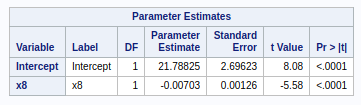
\includegraphics[width=.5\textwidth]{img/montgomery/procreg.png}
    \caption{Estimadores y p-valores para la regresión.}
    \label{img:mont-procreg}
  \end{figure}

  \paragraph{}
  Como podemos ver, el \textit{p-valor} para $\beta_1$ está por debajo de $0,05$, por lo que podemos rechazar la hipótesis nula con una confianza del 95\%. El \textit{p-valor} para el intercepto también permite rechazar la hipótesis nula.

  \paragraph{}
  Por tanto, los estimadores son:

  \begin{align}
    \hat\beta_0 = 21.78825\\
    \hat\beta_1 = -0.00703
  \end{align}

  \paragraph{}
  Con la recta de regresión:

  \begin{equation}
    y_i = 21.78825 -0.00703{x_8}_i + \varepsilon_i
  \end{equation}

  \paragraph{}
  La interpretación de estos parámetros es que con 0 yardas ganadas por el contrario, un equipo gana de media $21,78825$ juegos, y que por cada yarda que gana el contrario, el equipo pierde de media $0.00703$ juegos.

  \begin{figure}[H]
    \centering
    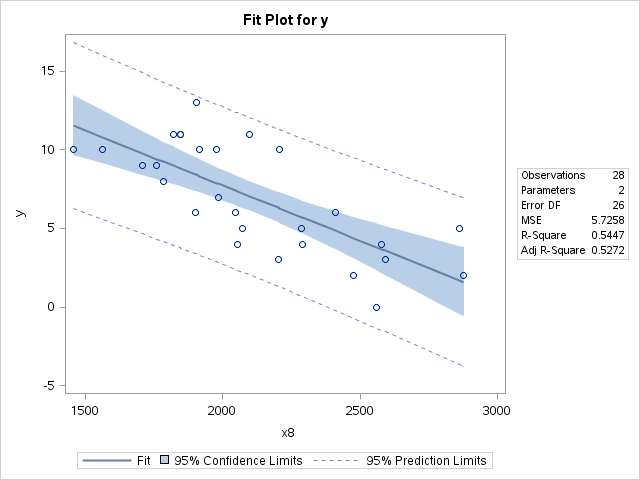
\includegraphics[width=.8\linewidth]{img/montgomery/fitplot.png}
    \caption{Fit plot del modelo de regresión lineal simple}
    \label{img:mont-fitplot}
  \end{figure}

  \subsubsection{Formar la tabla de análisis de varianza y probar el significado de la regresión.}

  \paragraph{}
  La tabla de análisis de la varianza se obtiene también mediante el procedimiento \textit{REG}.

  \begin{figure}[H]
    \centering
    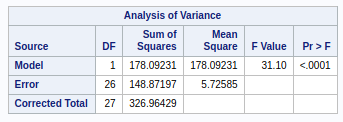
\includegraphics[width=.5\linewidth]{img/montgomery/anovatable.png}
    \caption{Tabla de análisis de la varianza}
    \label{img:mont-anova}
  \end{figure}

  \paragraph{}
  Esta tabla nos permite obtener la suma de cuadrados del modelo y del error, lo cual nos da un modo alternativo de hacer el contraste sobre el coeficiente $\beta_1$. \textit{Mean Square} para el \textit{Error} es el estimador de la varianza $\sigma^2$ obtenida por el error aleatorio $\varepsilon$. Si se cumple la hipótesis $H_0: \beta_1=0$, \textit{Mean Square} para el \textit{Model} también es un estimador de la varianza $\sigma^2$. Por tanto

  \begin{equation}
    F = \frac{MSM}{MSE}
  \end{equation}

  \paragraph{}
  es un estadístico que permite realizar el test de hipótesis sobre la hipótesis nula $H_0$. Esta tabla también nos proporciona el \textit{p-valor} para este contraste, que es menor que $0,05$, por lo que podemos rechazar la hipótesis, y afirmar que existe regresión con un 95\% de confianza.

  \subsubsection{Determinar un intervalo de confianza de 95\% para la pendiente.}

  \paragraph{}
  La pendiente es el parámetro $\beta_1$, y podemos obtener los intervalos de confianza para los parámetros mediante el procedimiento \textit{REG}, añadiendo la opción \textit{CLB} al modelo.

  \begin{figure}[H]
    \centering
    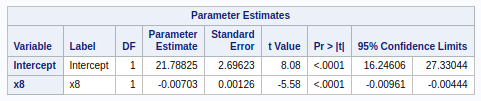
\includegraphics[width=.6\linewidth]{img/montgomery/icestim.png}
    \caption{Estimadores para los parámetros con intervalos de confianza del 95\%}
  \end{figure}

  \paragraph{}
  El intervalo de confianza de la pendiente es el correspondiente al parámetro $x_8$, por lo que la pendiente se situa entre $-0.00961$ y $-0.00444$.

  \subsubsection{?`Qué porcentaje de variabilidad total da $y$, y explica este modelo?}

  \paragraph{}
  Para obtener la medida de variabilidad total de $y$ debemos volver a la tabla de análisis de varianza del apartado \textbf{b}:

  \begin{figure}[H]
    \centering
    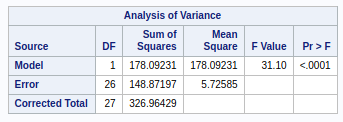
\includegraphics[width=.5\linewidth]{img/montgomery/anovatable.png}
    \caption{Tabla de análisis de la varianza}
  \end{figure}

  \paragraph{}
  Esta tabla nos da la \textit{Suma de cuadrados total}, que en este caso es igual a $326,96429$. Para obtener la variabilidad de la muestra, conocida como $MST$, se divide este valor por sus grados de libertad, que son $N-1$, siendo $N$ el número de observaciones.

  \begin{equation}
    MST = \frac{SST}{N-1} = \frac{326,96429}{27} = 12.109788519
  \end{equation}

  \paragraph{}
  Este valor $MST$ es la variabilidad total de la muestra $\sigma_T^2$, parte de la cual intentamos explicar mediante el modelo de regresión lineal simple. Existirá otra parte explicada por el error aleatorio, $\sigma^2$.

  \paragraph{}
  Para calcular la cantidad de variabilidad que explica el modelo podemos calcular:

  \begin{equation}
    \frac{SS_{Modelo}}{SS_{Total}}
  \end{equation}

  \paragraph{}
  Que es un coeficiente conocido como $R^2$, que también podemos obtener directamente con la siguiente tabla obtenida del procedimiento \textit{REG}:

  \begin{figure}[H]
    \centering
    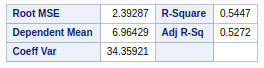
\includegraphics[width=.35\linewidth]{img/montgomery/tablaregaux.png}
    \caption{Coeficientes de la Regresión Lineal Simple.}
    \label{img:mont-tabla-aux}
  \end{figure}

  \paragraph{}
  \textit{R-square} indica que el modelo de regresión explica un $54.47\%$ de la variabilidad. También puede interpretarse como un indicador de cómo de bien se ajustan los datos a la línea de regresión ajustada.


  \subsubsection{Determinar un intervalo de confianza de 95\% para la cantidad promedio de juegos ganados, si la distancia ganada por tierra por los contrarios se limita a 2000 yardas.}

  \paragraph{}
  Este apartado nos pide hacer una predicción de $y$ cuando $x_8=2000$. Este valor no se encuentra entre nuestras observaciones, pero si que está dentro del rango definido por el mínimo y el máximo de $x_8$ para las observaciones, por lo que podremos realizar esta predicción. Añadiremos manualmente a los datos una observación en la que solo rellenamos el valor de $x_8$. \textit{SAS} realizará la predicción sobre el valor de la variable dependiente $y$ para este valor de $x_8$ dado el modelo de regresión conseguido mediante las observaciones completas.

  \paragraph{}
  Para mostrar los intervalos de confianza para las predicciones, añadimos la opción \textit{CLI} al modelo del procedimiento \textit{REG}.

  \begin{figure}[H]
    \centering
    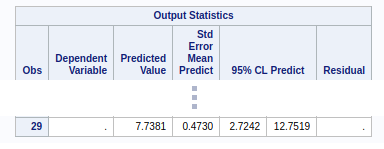
\includegraphics[width=.5\linewidth]{img/montgomery/prediccion2000.png}
    \caption{Intervalo de confianza del 95\% para la predicción de $x_8=2000$.}
    \label{img:mont-prediccion2000}
  \end{figure}

  \paragraph{}
  Como podemos ver, el valor predicho medio es $7,7381$ juegos ganados, y podemos afirmar con una confianza del 95\% que el valor real está entre $2,7242$ y $12,7519$ juegos ganados.

  \subsection{Supóngase que se quiere usar el modelo desarrollado en el problema 2.1 para pronosticar la cantidad de juegos que ganará un equipo si puede limitar los avances por tierra de sus contrarios a 1800 yardas. Determinar un estimado de punto de la cantidad de juegos ganados cuando $x_8=1800$. Determinar un intervalo de predicción de $90$ por ciento para la cantidad de juegos ganados.}

  \paragraph{}
  Como el apartado \textbf{2.1.e}, este ejercicio requiere hacer una predicción de $y$. El valor de $x_8$ pedido no está en las observaciones, pero se encuentra en el rango definido por el mínimo y el máximo de observaciones para $x_8$. Añadimos una observación con valor $x_8=1800$, al igual que hicimos para el anterior apartado, para el cual \textit{SAS} realizará una predicción de $y$ dado el modelo de regresión simple. Para conseguir el intervalo del 90\% de confianza, definimos en las opciones del modelo el \textit{ALPHA} como igual a $0.1$.

  \begin{figure}[H]
    \centering
    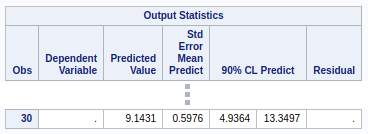
\includegraphics[width=.5\linewidth]{img/montgomery/prediccion1800.png}
    \caption{Intervalo de confianza del 90\% para la predicción de $x_8=1800$.}
    \label{img:mont-prediccion1800}
  \end{figure}

  \paragraph{}
  El estimado de punto es $9,1431$ juegos ganados, y el intervalo nos permite afirmar con un 90\% de confianza que el valor real está entre $4,9364$ y $13,3497$ juegos ganados.


  \part{Código Fuente}

    \begin{figure}[H]
      \centering
      \begin{minted}[frame=single,framesep=5pt]{sas}
filename reffile '/folders/myshortcuts/sas/regression-group-task/data/CH01PR20.csv';

proc import datafile=reffile dbms=csv out=copiers;
  getnames=yes;
run;

proc print data=copiers;
run;
      \end{minted}
      \caption{\emph{Código SAS:} Mantenimiento de Copiadoras - Importación del conjunto de datos.}
      \label{code:sas-copiers-1}
    \end{figure}


    \begin{figure}[H]
      \centering
      \begin{minted}[frame=single,framesep=5pt]{sas}
proc reg data=copiers;
  model y=x /clb alpha=0.1;
  id x;
run;
      \end{minted}
      \caption{\emph{Código SAS:} Mantenimiento de Copiadoras - Modelo de regresión simple.}
      \label{code:sas-copiers-2}
    \end{figure}

    \begin{figure}[H]
      \centering
      \begin{minted}[frame=single,framesep=5pt]{sas}
data copiers_new_observation;
  x = 5;
run;

proc append base=copiers data=copiers_new_observation;
run;

proc reg data=copiers;
  model y = x /r clm;
  id x;
run;
      \end{minted}
      \caption{\emph{Código SAS:} Mantenimiento de Copiadoras - Predicción para $X = 5$.}
      \label{code:sas-copiers-3}
    \end{figure}

    \begin{figure}[H]
      \centering
      \begin{minted}[frame=single,framesep=5pt]{sas}
data copiers_new_observation;
  x = 6;
run;

proc append base=copiers data=copiers_new_observation;
run;

proc reg data=copiers;
  model y = x /r cli clm alpha=0.1;
  id x;
run;
      \end{minted}
      \caption{\emph{Código SAS:} Mantenimiento de Copiadoras - Predicción para $X = 6$.}
      \label{code:sas-copiers-4}
    \end{figure}

    \begin{figure}[!h]
      \centering
      \begin{minted}[frame=single,framesep=5pt]{sas}
FILENAME REFFILE '/folders/myfolders/data-table-B1.XLS';

PROC IMPORT DATAFILE=REFFILE
  DBMS=XLS
  OUT=WORK.IMPORT;
  GETNAMES=YES;
RUN;

DATA FUTBOL;
  SET IMPORT;
  DROP X1 X2 X3 X4 X5 X6 X7 X9;
RUN;
      \end{minted}
      \caption{\emph{Código SAS:} Ejercicio 2.1 del Montgomery - Importación y preprocesado del conjunto de datos.}
      \label{code:sas-mont-1}
    \end{figure}


    \begin{figure}[!h]
      \centering
      \begin{minted}[frame=single,framesep=5pt]{sas}
PROC REG DATA=FUTBOL;
  MODEL Y=X8/CLB;
RUN;
      \end{minted}
      \caption{\emph{Código SAS:} Ejercicio 2.1 del Montgomery - Programa de Regresión Lineal Simple con intervalo para los parámetros.}
      \label{code:sas-mont-2}
    \end{figure}

    \begin{figure}[!h]
      \centering
      \begin{minted}[frame=single,framesep=5pt]{sas}
DATA AUX;
  INPUT X8;
  CARDS;
  2000
  1800
RUN;

PROC APPEND BASE=FUTBOL DATA=AUX; RUN;
      \end{minted}
      \caption{\emph{Código SAS:} Ejercicio 2.1 y 2.2 del Montgomery - Addición de valores para predicción.}
      \label{code:sas-mont-3}
    \end{figure}

    \begin{figure}[!h]
      \centering
      \begin{minted}[frame=single,framesep=5pt]{sas}
PROC REG DATA=FUTBOL;
  MODEL Y=X8/CLI;
RUN;
      \end{minted}
      \caption{\emph{Código SAS:} Ejercicio 2.1 del Montgomery - Obtención de valores predichos con intervalos de confianza del 95\%.}
      \label{code:sas-mont-4}
    \end{figure}

    \begin{figure}[!h]
      \centering
      \begin{minted}[frame=single,framesep=5pt]{sas}
PROC REG DATA=FUTBOL;
  MODEL Y=X8/CLI ALPHA=0.1;
RUN;
      \end{minted}
      \caption{\emph{Código SAS:} Ejercicio 2.2 del Montgomery - Obtención de valores predichos con intervalos de confianza del 90\%.}
      \label{code:sas-mont-5}
    \end{figure}

  %-----------------------------
  %  Bibliographic references
  %-----------------------------

  \nocite{rano2017}
  \nocite{sas}
  \nocite{neter1996applied}
  \nocite{montgomery2012introduction}

  \bibliographystyle{acm}
  \bibliography{bib}

\end{document}
